\documentclass{article}

\renewcommand{\thesection}{\Roman{section}}
\renewcommand{\thesubsection}{\thesection.\Roman{subsection}}

\usepackage[utf8]{inputenc}
\usepackage[tocindentauto]{tocstyle}
\usepackage[hidelinks]{hyperref}
\usepackage{latexsym,amssymb,amsmath,mathtools}
\usepackage{subcaption,float}
\usepackage{titling}
\usepackage{siunitx}
\usepackage{pdflscape}
\usepackage{eso-pic}
\usepackage{picture}
\usepackage{pdfpages}
\usepackage{tikz}
\usetikzlibrary{automata, positioning, arrows}
\usepackage{float}
\usepackage{minted}
\usepackage{pgfgantt}


\renewcommand\maketitlehooka{\null\mbox{}\vfill}
\renewcommand\maketitlehookd{\vfill\null}

\usepackage{sectsty}
\allsectionsfont{\normalfont\sffamily\bfseries}


\addtolength{\jot}{1em}


\usepackage{geometry}
\geometry{
    letterpaper,
    hmargin=3cm,
    vmargin=2cm,
}


\begin{document}

\begin{center}
    \sffamily{
        \textbf{
            \Huge{Alarm Clock Project}\\
            \vspace{0.5em} \huge{ECE 299}}\\
        \vspace{1em} August  18, 2020\\
    }
    \vspace{2em}
    
\includegraphics[width=1.43cm]{uvic_logo.png}\\
    \vspace{4em}
    \textbf{Group Information}\\
    Lab Section -- \textit{B03}\\
    Ben Kellman -- \textit{V00898289}\\
    Adam Carloni --\textit{V00886669}
\end{center}
\vspace{5em}
\begin{table}[h]
\centering
\begin{tabular}{c|c}
   &   Sections Responsible for\\\hline
 Ben  & Summary, VI, IV, Appendix A-D\\
 Adam & I,II,VI, V, VII
\end{tabular}
\end{table}

\AddToShipoutPicture*{
  \AtPageLowerLeft{
    \makebox(\paperwidth,0)[rb]{
\includegraphics{uvic_corner_logo.jpg}}%
  }
}

\pagenumbering{gobble}
\newpage


\section*{Executive Summary}
\paragraph{}
This report details the design of an alarm clock created as part of ECE299. The alarm clock displays the current time on an LCD display in a 24h format. It also features snooze functionality and an LCD backlight that will turn on or off based on the ambient light levels. The user accesses these features through an intuitive user interface, that features an LCD display and 6 input buttons. Due to the COVID-19 pandemic, most of the project was designed and using the Tinkercad circuit simulator. The one exception to this being the printed circuit board that was designed in KiCad and manufactured by JLCPCB. Overall, the project was successful. The only major error was a short circuit in the printed circuit board.  Creating a checklist of things to check/do before ordering the final printed circuit board would have prevented this.


\addcontentsline{toc}{section}{Executive Summary}
\pagenumbering{roman}
\newpage
\tableofcontents
\newpage
\listoftables
\addcontentsline{toc}{section}{List of Tables}
\newpage
\listoffigures
\addcontentsline{toc}{section}{List of Figures}
\newpage

\pagenumbering{arabic}
\section{Project Goal} %Adam
\paragraph{}
To use our skills and knowledge to create a functional alarm clock using an Arduino UNO R3 with our own PCB design. The alarm clock must allow a user to change the time, set and disable an alarm and have a snooze function. Additionally, the display brightness should adjust based on the current light level so it is always readable.

\section{Constraints} %Adam
\paragraph{}
Several hardware, software and logistical constraints were imposed on this project. The following section provides a detailed overview of these constraints.

\subsection{Hardware}
\paragraph{}
The main hardware constraints of this project were: the need to use an Arduino and the restriction of only using components available in Tinkercad. The Arduino Uno has several hardware limitations that affected the project. First, the GPIO (general purpose input-output) pins use 5V logic\cite{arduino}, meaning all components must also run off 5V logic. The Arduino is also limited to sourcing/sinking 20mA per GPIO pin\cite{arduino} (the Atmega328p can source/sink up to 40mA per pin\cite{atmega}, but this is not recommended). The total current source by GPIO pins is also limited to 200mA according to section 28.1 of the Atmega328p datasheet\cite{atmega}. As this project was simple, only using Tinkercad components was not a significant limitation.

\subsection{Software}
Most of the software constraints come from using an Arduino Uno in Tinkercad. The Arduino has 32kB (flash) memory available for program code and 2kB of static ram (SRAM) available for local and global variables\cite{arduino}. This was not a significant limitation as the final code only used ~10kB of the flash memory and ~0.5kB of the SRAM was statically allocated. The Arduino compiler in Tinkercad also only appears to support a subset of C++98, while the current Arduino IDE supports C++11. This prevents the use of some more modern C++ features such as nullptr in the project. Additionally, the Tinkercad compiler does not allow any user-defined types as function parameters and some calls to sprintf seem to break the simulation. These issues are not present when using the current Arduino IDE (1.8.8) and a physical Arduino.

\subsection{Logistical}
Several other constraints were present from course requirements and COVID-19. Due to COVID 19, all project work had to done remotely using tools such as Zoom for communication. This also restricted all prototyping to Tinkercad simulations, instead of prototyping on a breadboard. Additionally, the total cost of the project should be under \$100 per developer (total of \$200). This was so a physical copy of the alarm clock could be made by the group at the end of the course. A summary of the project timeline is shown in Appendix D as gantt chart.


% \begin{itemize}
%     \item Budget of no more than \$100 per developer (total of \$200)
%     \item Each developer works virtually from home
%     \item Use of Arduino Uno R3 with C++ coding
%     \item Limited to testing via TinkerCAD and KiCAD prior to assembly and for demonstration
%     \item Size of alarm clock must be able to fit nicely on a standard bedside nightstand
%     \item Button placement to be easily accessible to change time
%     \item Clock should continue to display time while alarm/snooze is triggered
%     \item Button pressing should not create a debounce effect
%     \item Brightness of the alarm clock to be auto-adjusted via ambient light
%     \item Soldering (limited experience)
%     \item Design of enclosure via Solidworks (limited experience)
%     \item Design of enclosure via solidworks (limited experience)
% \end{itemize}

% \subsection{Timeline}

% The timeline for tasks to completed are the following:

% \begin{itemize}
%     \item July 10 - Research; thorough understanding of what parts we need to order and how the software will work
%     \item July 12 – Electrical schematic; completed via KiaCAD with all parts and footprints labeled and wired
%     \item July 20 - Software; main program to be "generally" completed with fine tuning to be adjusted prior to Project Demonstration
%     \item July 24 - PCB completed and ordered; dimensions of all buttons and layout for enclosure design
%     \item July 26 - Enclosure design; via Solidworks matching the dimensions of all components and layout of PCB
%     \item July 27 - Project demonstration via TinkerCAD; to show T.A. in lab session working virtual alarm clock as per all requirements
%     \item August 18 - Final report due; submitted via coursespaces
%     \item August 20 - Enclosure made; laser cut acrylic to exact dimensions of PCB and button layout via Solidworks
%     \item August 21 - Alarm Clock completion; successful build of a working alarm clock as per all requirement specifications
% \end{itemize}


\section{Requirement Specifications} %Adam
\paragraph{}
The following project requirements where given to us to satisfy\cite{slides}. The alarm clock must
\begin{itemize}
    \item Allow user to set the time
    \item Display the current time in 24h format
    \item Allow the user to set and change the alarm time
    \item Allow the user to disable the alarm
    \item Allow the user to snooze the alarm
    \item Change the display brightness based on the ambient light levels
\end{itemize}
The rest of this section details a detailed list of requirements specification that where created by the design group to ensure the Alarm clock functions optimally.

\subsection{Hardware}
The following hardware requirements were determined to ensure the Alarm clock can be operated safely and easily:
\begin{itemize}
    \item Current draw must be limited to 20mA for all GPIO pin\cite{arduino}.
    \item Total current sourced by GPIO pins must be under 200mA \cite{atmega}.
    \item Alarm should produce a sound at a frequency of 3kHz (as human ears are most sensitive frequencies in this range \cite{human}).
    \item The alarm should produce a sound of around 70dB as prolonged exposure to sounds above 85dB can cause hearing damage \cite{linkbc}, so this is a good compromise between being loud and safe \cite{loud}.
    \item All components must be 5V tolerant, so they can be powered directly from the Arduino.
    \item The total enclosure must have a footprint that is smaller than 200mm$\times$200mm, as most night stands are ~450mm$\times$450mm\cite{nightstand}. This allows room for other objects, such as a lamp, on the nightstand.
    \item Button spacing should be at least 13mm due to the average thickness of the human finger \cite{finger}.
    \item The PCB must be a 2 layer board that does exceed 100mm$\times$100mm to reduce the cost.
    \item The PCB must be RoHS compliant.
    \item The PCB must be manufacturable meaning that: Drill hole size between 0.20mm-6.30mm, Hole to hole clearance of 0.54mm, Via to via clearance of 0.254mm, Via to track (trace) of 0.254mm and Minimum trace width and spacing for 2 layer is 0.127mm \cite{mfn}.
\end{itemize}

\subsection{User Interface}
The following specification were determined to ensure the alarm clock is easy and intuitive of the user to use
\begin{itemize}
    \item Current time should be displayed whenever possible, even when alarm is active
    \item The alarm should be able to be disabled completely
    \item The display should always indicate if an alarm is set
    \item It should take the user less than a minute to change the time
    \item The user should be able to cancel the alarm while it is snoozing without waiting for the alarm to sound again
    \item The display must indicate when the alarm is snoozing
    \item The backlight should be able to be turned on and off manually or automatically
    \item The backlight should automatically turn on if the ambient light level is under 100 Lux (approximately the ambient light of a very dark day \cite{lux})
    \item The displayed characters should be at least 5mm tall on the display (so they can be seen from 1m away \cite{letter}) since the approximate reach of the average human arm is around 0.80m \cite{arm}.
    \item Buttons must be 'debounced' so a single press in not registered multiple times
\end{itemize}

% \subsection{Use of Arduino UNO R3}
% All relevant requirements for using the Aruino UNO R3 with other hardware to complete the project goal are listed from the manufacturer and is as follows \cite{arduino}:
% \begin{table}[h!]
%     \centering
%     \begin{tabular}{l|l}
%         \textbf{Requirement} & \textbf{Quantity} \\
%         \hline Operating Voltage & 5V \\
%         \hline Input Voltage Power Recommendation & 7-12V \\
%         \hline Input Voltage Power Limit & 6-20V \\
%         \hline Digital I/O Pins & 14 \\
%         \hline Analog Input Pins & 6 \\
%         \hline Current per I/O Pin & 20mA (Under 5V operation) \\
%         \hline Pin Operation Voltage & 0-5V \\
%         \hline Clock Speed & 16MHz \\
%         \hline Memory & 32KB \\
%         \hline Length & 68.6mm \\
%         \hline Width & 53.4mm \\

%     \end{tabular}
%     \caption{Arduino Requirement Specifications}
% \end{table}

% \paragraph{}
% If any hardware components that are used with the Arduino UNO R3 exceed these specifications, damage to the Arduino UNO R3 may result. For example, if the external power supplied to the Arduino UNO R3 is more than the input voltage power limit (20V), the voltage regulator may overheat. Another specification to watch for is if any of the I/O pins pass more than 20mA, the pin may permanently fail and might also cause damage to the micro-controller. This can be caused by overloading the pin with too much load, or accidentally shorting the "high" I/O pins to ground, and/or shorting I/O pins to each other.


% \subsection{Sound}
% The average human ear is most sensitive to frequencies between 2000-5000Hz and can typically hear sounds from 0 decibels and up \cite{human}. Standard alarm clocks on the market are about 70 to 80 decibels in loudness - which from a hearing standpoint are considered to be as loud as a busy street \cite{loud}. However, according to the Government of British Columbia, any prolonged sound above 85 decibels is considered harmful and can cause permanent hearing loss \cite{linkbc}. For these reasons, we will specify the \textbf{audio on the alarm be between 2000-5000Hz and 70-80 decibels}.

% \subsection{Time Display}
% [reword to make more clear on why picking the lcd and the stn - showing more information]. The type of display should be able to print clear letters as well as numbers for user convenience and programming ease. With the average reach distance of 80cm of human arm \cite{arm}, we will specify that the \textbf{user should still clearly see the digits and letters on the display from 100cm, or 1 meter, away}. In order to satisfy this, \textbf{letter height should be a minimum of 5mm on the display} \cite{letter}. For this reason, a cost effective STN LCD display is preferred over any segmented display or expensive high resolution LED screen \cite{lcd1}. Further, the display shall not exceed any of the electrical specifications of section III.I and specifically have a power input rating of \textbf{5V} (do not want 2 external power sources or transformer as that would be an additional cost).

% \subsection{PCB}
% With the recommended PCB manufacturer being JLCPCB, some notable requirements are observed. Some of the requirements most relevant to this project are as follows \cite{mfn}:
%     \begin{itemize}
%         \item Dimension of PCB be \textbf{less than 100mm x 100mm} to be the most cost effective for our budget of under \$100 per developer
%         \item 1,2,4,6 copper layers on board; \textbf{2 copper layers is most cost effective}
%         \item Drill hole size between 0.20mm-6.30mm
%         \item Hole to hole clearance of 0.54mm
%         \item Via to via clearance of 0.254mm
%         \item Via to track (trace) of 0.254mm
%         \item Minimum trace width and spacing for 2 layer is 0.127mm
%     \end{itemize}

% \subsection{Brightness}
% The display brightness must be able to change via ambient light; increase when ambient light conditions are brighter and decrease when ambient light conditions are darker. Since the alarm clock is rated for indoor use, the ideal light intensity detection by a photo-transistor would be anywhere from 0 Lux (no light) to at less than 100 Lux (cloudy day) \cite{lux}.

% \subsection{Enclosure}
% With a standard night stand being around 18 inches (457.2mm) wide \cite{nightstand}, it is reasonable to require the closure be no more than \textbf{200mm} for any dimension (L/W/H) as to make room for other objects, such as a night lamp. Further, the buttons on the enclosure are required to be no less than \textbf{13mm apart} for user ease of use due to the average thickness of human index finger tip \cite{finger}.

\begin{landscape}
\thispagestyle{empty}

\section{Bill of Materials} %Ben
The bill of materials can be seen in Table \ref{tab:bom} and component choice justifications can be seen in Table \ref{tab:just}.
\begin{table}[h!]
    \centering
    \begin{tabular}{l|l|l|c|c|c|l}
    \textbf{Designator(s)}&\textbf{Manufacturer Part   Number} & \textbf{Digi-Key Link} & \textbf{Quantity} & \textbf{Unit Price} & \textbf{Extended Price} & \textbf{Description}      \\
    \hline
RV1&P120PK-Y25BR10K                  & \href{https://www.digikey.ca/en/products/detail/tt-electronics-bi/P120PK-Y25BR10K/5957454}{\underline{987-1710-ND}}               & 1                 & 0.91                & \$0.91                  & 10K Pot                   \\
BZ1&PKM22EPPH2001-B0                 & \href{https://www.digikey.ca/en/products/detail/murata-electronics/PKM22EPPH2001-B0/1219322}{\underline{490-4691-ND}}             & 1                 & 1.12                & \$1.12                  & Piezo Buzzer              \\
PB2&RP3502MARED                      & \href{https://www.digikey.ca/en/products/detail/e-switch/RP3502MARED/280456}{\underline{EG1938-ND}}                               & 1                 & 4.84                & \$4.84                  & Large Panel Mount Button  \\
PB3&PS1024ALRED                      & \href{https://www.digikey.ca/en/products/detail/e-switch/PS1024ALRED/81539}{\underline{EG2025-ND}}                                & 1                 & 2.07                & \$2.07                  & Small Panel Mount Button  \\
PB1,PB4-6&2-1825910-7                & \href{https://www.digikey.ca/en/products/detail/te-connectivity-alcoswitch-switches/2-1825910-7/1632528}{\underline{450-1642-ND}} & 4                 & 0.18                & \$0.72                  & Tactile Switch            \\
R1&PDV-P9007                         & \href{https://www.digikey.ca/en/products/detail/advanced-photonix/PDV-P9007/480624}{\underline{PDV-P9007-ND}}                     & 1                 & 2.57                & \$2.57                  & Photo-resistor             \\
DS1&MOP-AL162A-BYFY-25J-3IN          & \href{https://www.digikey.ca/en/products/detail/matrix-orbital/MOP-AL162A-BYFY-25J-3IN/9602838}{\underline{635-1205-ND}}          & 1                 & 13.75               & \$13.75                 & 16X2 LCD                  \\
A1&A000073                           & \href{https://www.digikey.ca/en/products/detail/arduino/A000073/3476357}{\underline{1050-1041-ND}}                                & 1                 & 30.15               & \$30.15                 & Arduino Uno R3            \\
R2&RNMF14FTC5K60                    & \href{https://www.digikey.ca/en/products/detail/stackpole-electronics-inc/RNMF14FTC5K60/2617364}{\underline{S5.6KCACT-ND}}         & 1                 & 0.14                & \$0.14                  & 5.6K Resistor               \\
R3&RNMF14FTC47R0                     & \href{https://www.digikey.ca/en/products/detail/stackpole-electronics-inc/RNMF14FTC47R0/2617352}{\underline{S47CACT-ND}}          & 1                 & 0.14                & \$0.14                  & 47 Ohm Resistor          \\

    \hline
    &&&\textbf{Total}&\textbf{\$56.41}&
    \end{tabular}
    \caption{BoM}
    \label{tab:bom}
\end{table}

\begin{table}[h!]
    \centering
    \begin{tabular}{l|l}
        \textbf{Designator(s)} & \textbf{Reason} \\ \hline
        RV1                    & Recommended value from page 11 of the LCD datasheet\cite{lcd}\\\hline
        BZ1                    & Needed to generate alarm sound (3kHz and 70 decibels)\\\hline
        PB2                    & A large panel mount button for the snooze button, to distinguish it from the time setting buttons\\\hline
        PB3                    & A smaller panel mount button that can be used for the cancel alarm button (see appendix A for mounting details) \\\hline
        PB1,PB4-6              & Tactile switches for T+/T-/Backlight/Time Set buttons (13mm tall to reach through enclosure)\\\hline
        R1                     & Photo-resistor to detect ambient light (detects up to 100 Lux)\\\hline
        DS1                    & Has a character height of 5.95mm and allows more information to be displayed than a 7 segment display\\\hline
        A1                     & Arduion Uno, needed to implement all logic and time keeping\\\hline
        R2                     & Used to construct a voltage divider with photo-resistor\\\hline
        R3                     & Current limiting resistor for the display backlight
    \end{tabular}
    \caption{Component Choice Justifications}
    \label{tab:just}
\end{table}

\vfill
{\makebox[\linewidth]{\thepage}}
\end{landscape}


\section{Circuit Schematic \& PCB} %Adam
\paragraph{}
This section provides details about the circuit schematic and PCB created for this project.

\subsection{Circuit Schematic}
\paragraph{}
The circuit schematic used for the project can be seen on the next page. The exact components used can be found from their reference designators in the Bill of Materials in section IV. Note that:
\begin{itemize}
    \item The photo-resistor is configured as a voltage divider so that a varying analog voltage can be fed into the analog input pin A0
    \item Analog input pins A1-A4 are configured as digital inputs since the photo-resistor is the only component that requires an analog voltage
    \item The backlight is connected to connected to a PWM pin so it brightness could be varied (although this feature is not used by the alarm)
\end{itemize}

\subsection{Design Calculation}
The following section presents some brief design calculations used to choose resistor values.

\paragraph{Backlight Resistor} From the LCD datasheet, the voltage drop across the LCD backlight ranges from 4.2-4.6V and the maximum current is 120mA \cite{lcd}. Testing with the physical display showed that 20mA was sufficient to enable the display, so it can be driven from a GPIO pin. To ensure no more than 20mA is drawn from the GPIO pin, the resistor value can be found as:
\begin{align}
    R_{LCD} =\frac{V_{LED}}{I_{LED}}=\frac{5\si{V}-4.2\si{V}}{20\si{mA}}=50\si{\ohm}
\end{align}
\begin{enumerate}
    \item $R_{LCD}$ is the value of the current limiting resistor in $\si{\ohm}$
    \item $V_{LED}$ is the voltage drop across the backlight in V
    \item $I_{LED}$ is the current through the backlight in A
\end{enumerate}
Taking as standard resistor value we get that the current limiting resistor should be: $R_{LCD}=47\si{\ohm}$. This may result in a current slightly larger than 20mA. This is acceptable since the Atmega328p is rated for 40mA per GPIO pin, so sourcing slightly over 20mA should not cause any damage.

\paragraph{Voltage Divider Resistor} From the photo-resistor datasheet we can see that its resistance varies from ~$2\si{k\ohm}-9\si{k\ohm}$\cite{ldr} at 100 lux. Due to this wide range, precision sensing is not possible. To simplify the design value in the middle of the range was chosen: $R_{div}=5.6\si{k\ohm}$. This means when the ambient light levels are around 100 lux, the input voltage will be around 2.5V, leading to an ADC reading of 512.

\includepdf[landscape=true]{AlarmPCB.pdf}

% \paragraph{}
% Below is a close up look at the schematic of the 6 push buttons that will protrude out of the enclosure for user interface. They are all normally open with each one have a specific purpose, as labeled in the image below.
% \begin{figure}[H]
%     \centering
%     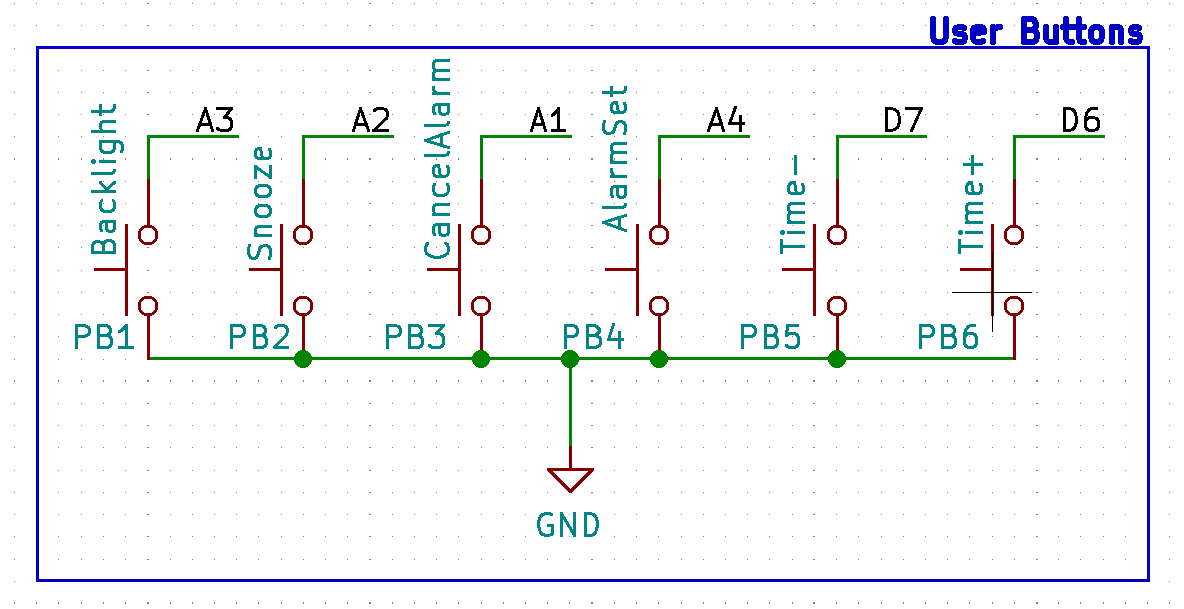
\includegraphics[width=\textwidth]{Schematic PB.PNG}
%     \caption{Circuit Schematic: User Buttons}
%     \label{fig:my_label}
% \end{figure}

% \newpage
% \paragraph{}
% A close up look at the Arduino schematic. As seen below:
% \begin{itemize}
%     \item 5V power supply at top
%     \item Ground connections as shown at bottom and where noted
%     \item Photoresistor (R1) to first analog input A0 with 2k resistor attached to ground
%     \item 4 of the user buttons mentioned above are being used by the next 4 analog inputs
%     \item I/O pins 2-5 and 10-12 are wired to control LCD functionality
%     \item I/O pins 6 and 7 are related to the time+ and time- buttons controlled by the user
%     \item I/O pin 9 controls the 70 decibel buzzer for alarm
% \end{itemize}
% \begin{figure}[H]
%     \centering
%     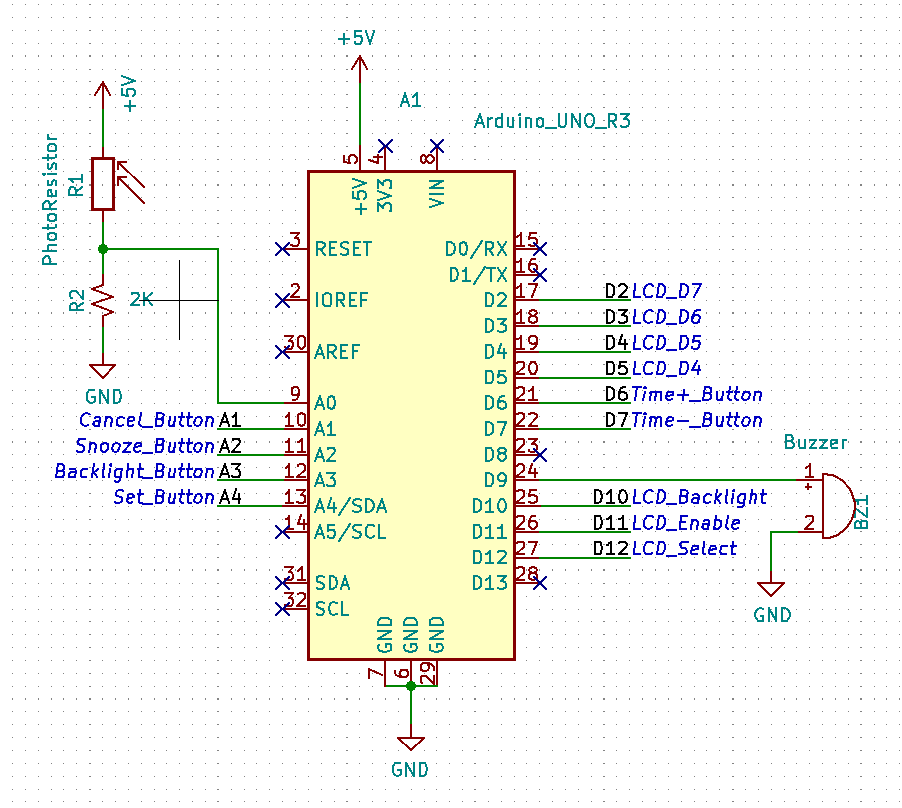
\includegraphics[width=\textwidth]{Schematic Arduino2.PNG}
%     \caption{Circuit Schematic: Arduino}
%     \label{fig:my_label}
% \end{figure}

% \newpage
% \paragraph{}
% Below is the LCD manufactures drawing and interface, which is used to map the corresponding pins to the Arduino to display time/alarm requirements.
% \begin{figure}[H]
%     \centering
%     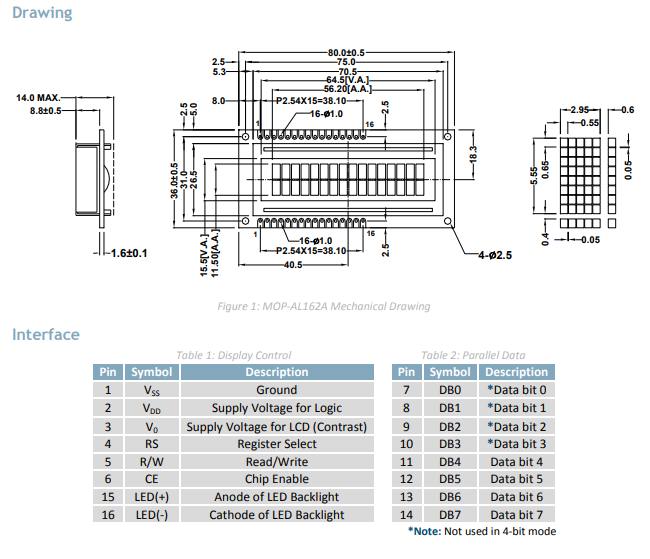
\includegraphics[width=\textwidth]{Schematic LCD Drawing.PNG}
%     \caption{Circuit Schematic: LCD Pin Mapping []}
%     \label{fig:my_label}
% \end{figure}

% \newpage
% \paragraph{}
% In accordance with the LCD pin mapping above, the LCD is wired to the Arduino as shown below. Note the contrast of the LCD is controlled by the user via potentiometer to pin 3.
% \begin{figure}[H]
%     \centering
%     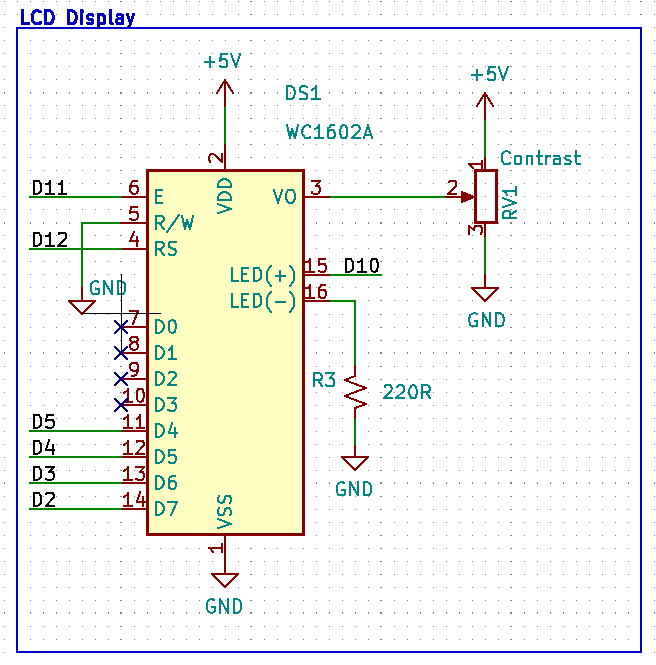
\includegraphics[width=\textwidth]{Schematic LCD.PNG}
%     \caption{Circuit Schematic: LCD}
%     \label{fig:my_label}
% \end{figure}

\subsection{PCB}
The PCB layout can be seen in Figure \ref{fig:layout}. Note that:
\begin{itemize}
    \item The 4 user buttons - spaced 13mm apart - at the top of the PCB (Time+, Time-, Alarm Set, and Backlight) protrude out of the enclosure for user interface.
    \item The Snooze button and Cancel Alarm button are mounted on enclosure and connected to the PCB via wires.
    \item GND planes are used on the top an bottom of the PCB to improve signal integrity and simplify routing
    \item The trace connecting Pin 16 of the LCD to R3 is shorted to Pin A0 of the Arduino, this is not intended and is design error
\end{itemize}
\begin{figure}[H]
    \centering
    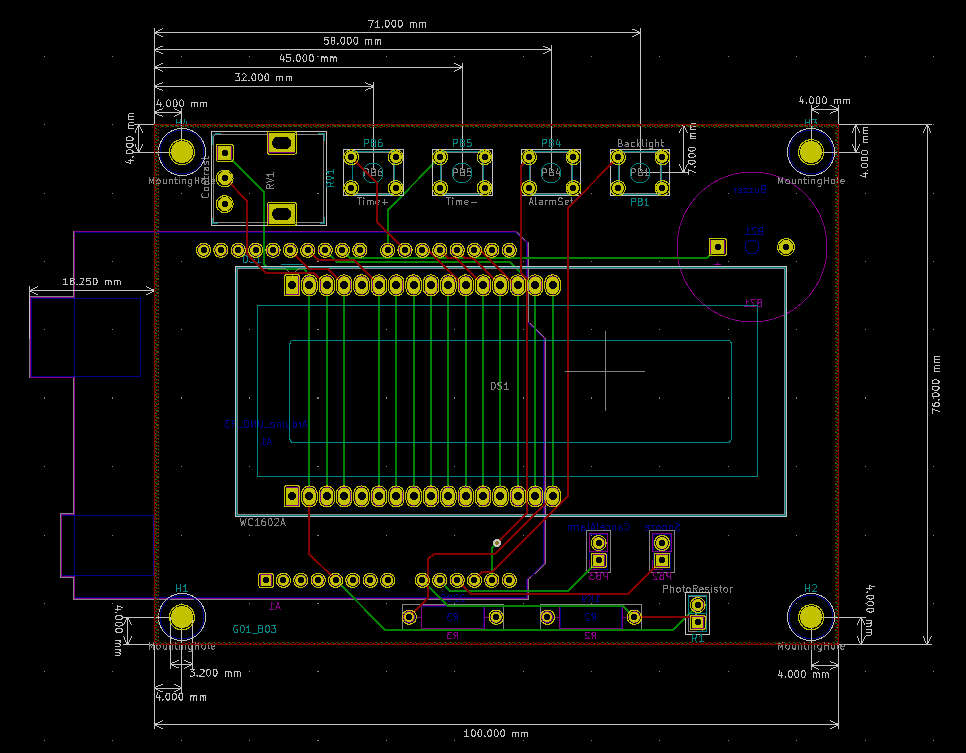
\includegraphics[width=\textwidth]{pcb_layout.png}
    \caption{PCB Layout}
    \label{fig:layout}
\end{figure}

\newpage
Some more views of the PCB can be seen in Figure \ref{fig:more_pcb}
\begin{figure}[h]
    \centering
    \begin{subfigure}{0.4\textwidth}
        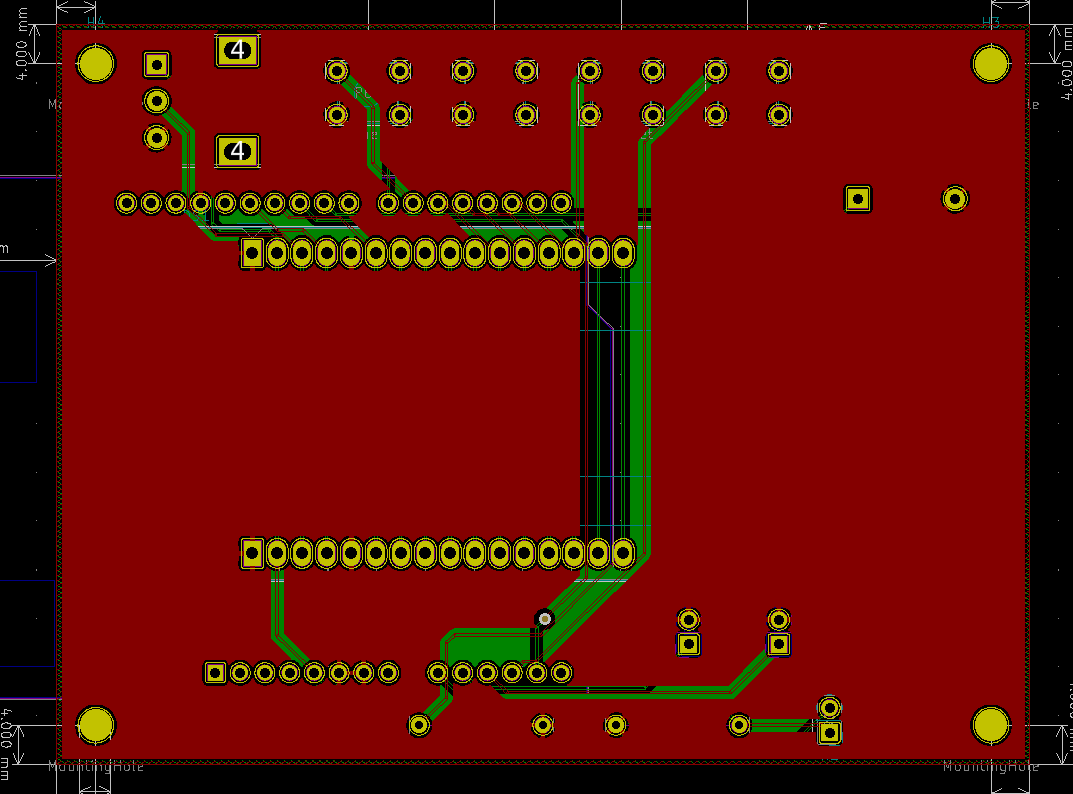
\includegraphics[width=\textwidth]{PCB_Front.PNG}
        \caption{PCB: Front Copper Side}
    \end{subfigure}
    \begin{subfigure}{0.4\textwidth}
        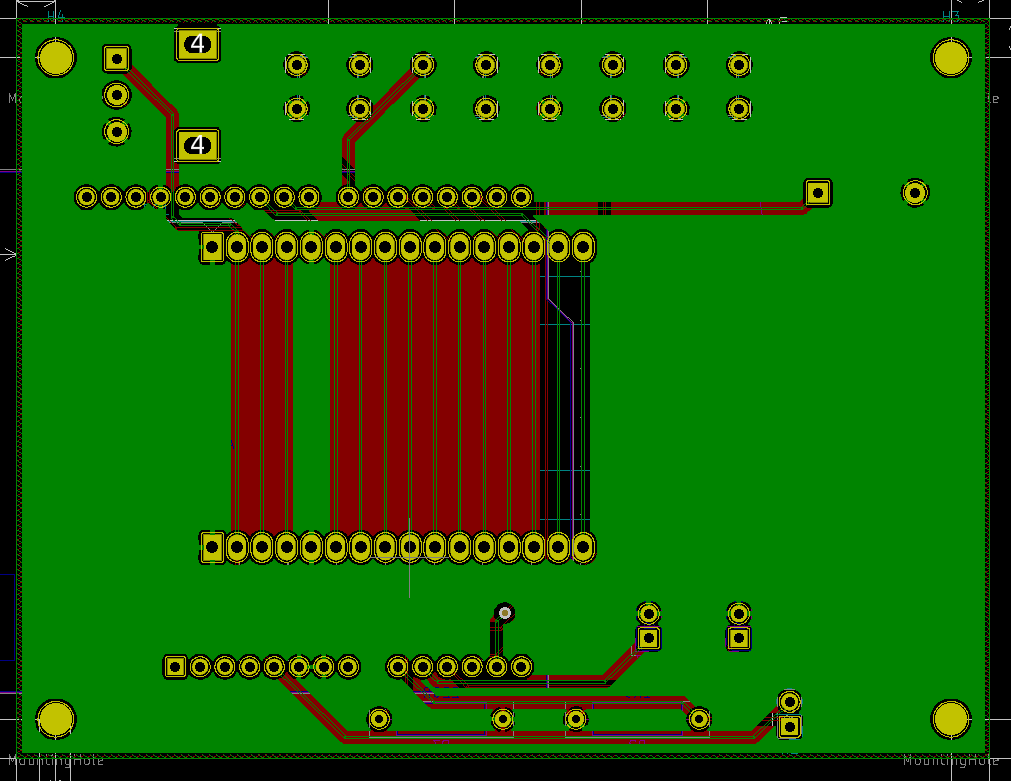
\includegraphics[width=\textwidth]{PCB_Back.PNG}
        \caption{PCB: Back Copper Side}
    \end{subfigure}
    \begin{subfigure}{0.4\textwidth}
        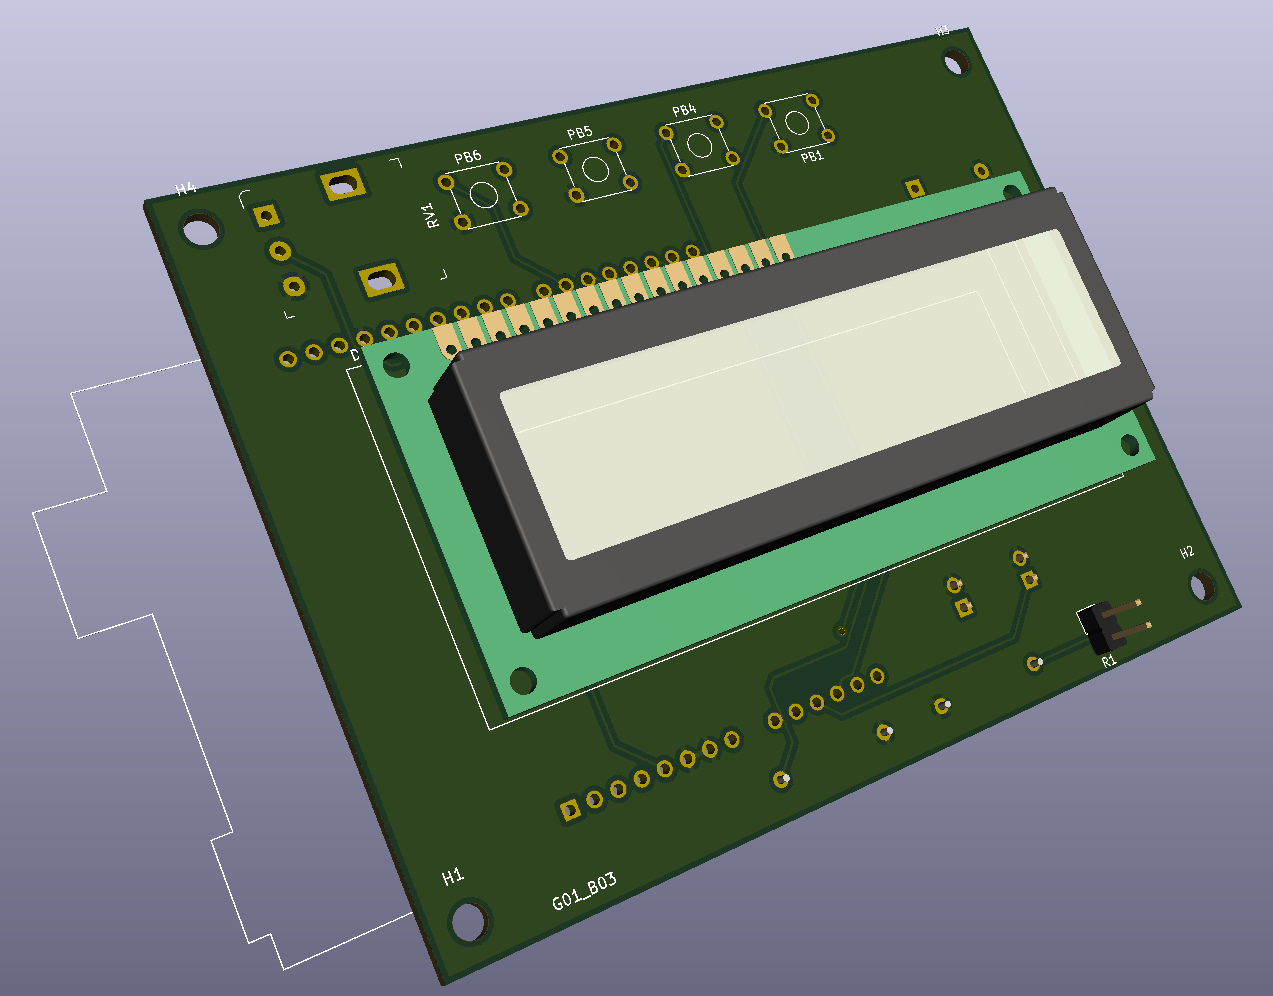
\includegraphics[width=\textwidth]{PCB_3D.PNG}
        \caption{PCB: Front 3D View}
    \end{subfigure}
    \begin{subfigure}{0.4\textwidth}
        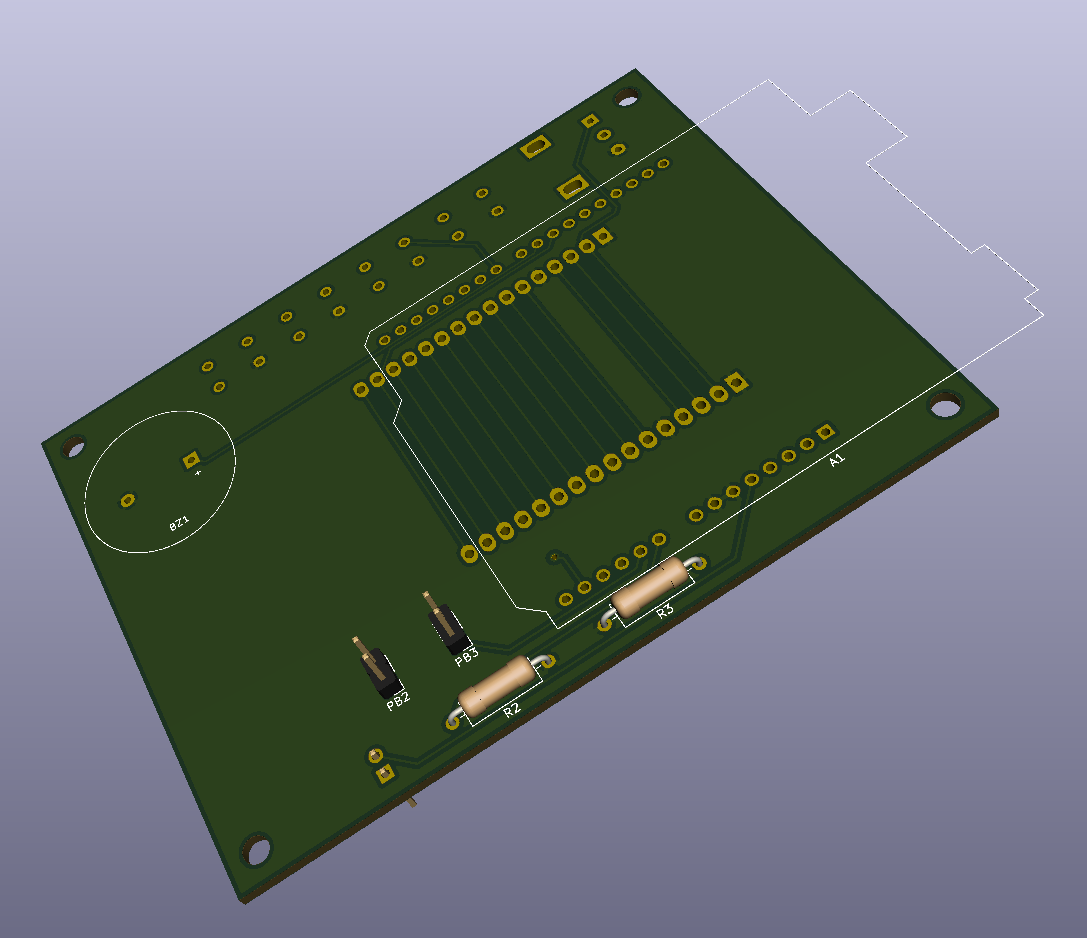
\includegraphics[width=\textwidth]{PCB_3D_Back.PNG}
        \caption{PCB: Back 3D View}
    \end{subfigure}


    \caption{Additional PCB layout views}
    \label{fig:more_pcb}
\end{figure}

\section{Testing \& Validation} %Ben
This section will cover the test procedures and results used to validate the alarm clock's operation. All tests were performed in tinkercad.

\subsection{Testing Limitations}
\paragraph{}
Since all testing needed to be performed in Tinkercad, there were some major limitations, particularly in the hardware test section. The backlight of the LCD display in Tinkercad has a different voltage drop and maximum current than the one sourced for the project. This means the current measured in Tinkercad may not reflect the actual current drawn by the design. The actual current draw could be greater than 20mA. Although, would likely be acceptable as the Atmega328p is capable of sourcing up to 40mA\cite{atmega} so a current draw slightly over 20mA should not damage it. The photo-resistor used also has different characteristics that the one used in Tinkercad, so it is simulated with fixed value resistors for the purposes of testing functionality surrounding it.

\begin{landscape}
\thispagestyle{empty}

\subsection{Hardware}
Hardware testing consists of verifying all components function properly and within tolerances. The test matrix shown in Table \ref{tab:hw_test} was executed in Tinkercad using the circuit presented in section V with the code listed in Appendix B running on the Arduino. All current measurements are made using an ammeter in series with the component, the total current was estimated by an ammeter in series with the GND pin of the Arduino.

\begin{table}[h!]
    \centering
    \begin{tabular}{|p{0.15\textwidth}|p{0.3\textwidth}|p{0.4\textwidth}|p{0.2\textwidth}|p{0.1\textwidth}|}
    \hline
       Name & Description & Expected Result & Result & Pass/Fail\\
       \hline
       LCD Display& Verify Text can be displayed&"Hello World" should be displayed&"Hello World"&Pass\\\hline
       LCD Backlight& Verify Backlight turns on& Backlight should blink&Backlight Blinking&Pass\\\hline
       Backlight Current& & Backlight should draw less than 20mA & 15.3mA & Pass\\\hline
       LCD Contrast& Verify Pot Adjust Contrast& Turning Pot should adjust LCD Contrast& Expected& Pass\\\hline
       Buzzer Sound& Verify Buzzer Sounds &Buzzer should sound periodically& Expected& Pass\\  \hline
       Buzzer Current& Verify buzzer does not draw too much current& Current should be under 20mA& 3.84mA& Pass\\\hline
       Photoresistor& Verify photo resistor voltage is read by Arduion& Number second line of the LCD should change with light & Expected & Pass\\\hline
       AlarmSet \newline Button& Verify Button Works& 'AlarmSet' should print on serial\newline terminal when button is pressed &Expected & Pass\\\hline
       T- Button& Verify Button Works& 'T-' should print on serial\newline terminal when button is pressed &Expected & Pass\\\hline
       T+ Button& Verify Button Works& 'T+' should print on serial\newline terminal when button is pressed &Expected & Pass\\\hline
       Backlight\newline Button& Verify Button Works& 'Backlight' should print on serial\newline terminal when button is pressed &Expected & Pass\\\hline
       Snooze \newline Button& Verify Button Works& 'Snooze' should print on serial\newline terminal when button is pressed &Expected & Pass\\\hline
       Cancel Alarm \newline Button& Verify Button Works& 'Cancel' should print on serial\newline terminal when button is pressed &Expected & Pass\\\hline
       Total Current& &Total GPIO current less than 200mA& 21.1mA& Pass\\
       \hline
       &\textbf{Overall Result} &&& \textbf{Pass}\\
       \hline
    \end{tabular}
    \caption{Hardware Test Matrix}
    \label{tab:hw_test}
\end{table}
\vfill
{\makebox[\linewidth]{\thepage}}
\end{landscape}
The actual test setup can be seen in the figure below.
\begin{figure}[h]
    \centering
    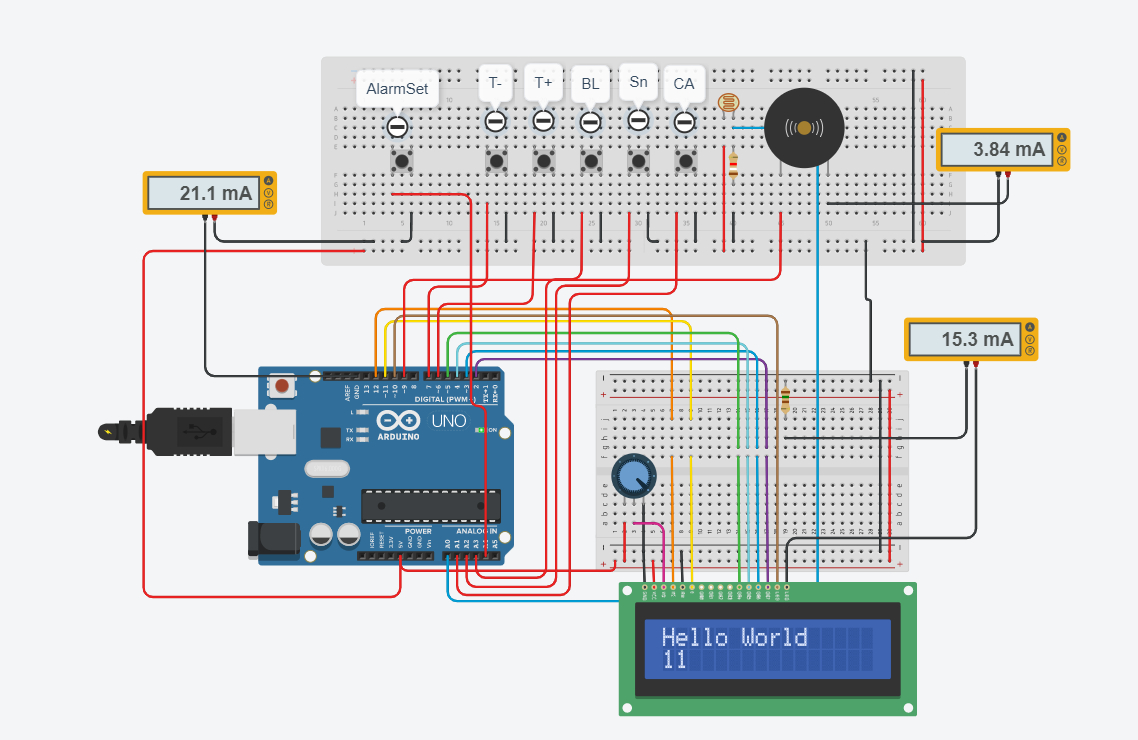
\includegraphics[width=0.8\textwidth]{TestSetup.png}
    \caption{Test Setup in Tinkercad}
    \label{fig:test}
\end{figure}

\subsection{Firmware}
The following section presents the tests and results used to validate the firmware's behaviour. These tests ensure that all the specified behaviour works correctly. A finite state machine diagram can be seen below to illustrate the general functionality of the alarm.

\begin{figure}[h!]
    \centering
    
\includegraphics[width=0.8\textwidth]{fsm.png}
    \caption{FSM Diagram}
    \label{fig:fsm}
\end{figure}

The following table presents the definitions of the state transitions conditions. A press/release corresponds to the button being pressed down or released once. If a nc is present after a condition it means that it will not be cleared (ie. on entering the next state a button will still register as being pressed or released).
\newpage
\begin{table}[h]
    \centering
    \begin{tabular}{l|l}
        \textbf{ID} & \textbf{Description}\\\hline
        Inc\_P &  T+ or T- has been pressed\\
        Inc\_R &  T+ or T- has been released\\
        As\_P  &  Alarm Set has been pressed\\
        Bl\_P  &  Backlight has been pressed\\
        Ca\_P &   Cancel Alarm has been pressed\\
        Sn\_P &   Snooze has been pressed\\
        Sn\_Exp & Clock has been in snooze state for more than 2 mins\\
        AL\_T &  The current time equals the alarm time (only checks hours and minuets)\\
        Slw\_t\_Fst & At least 1 increments have been made in slow mode and the last minute digit is zero
    \end{tabular}
    \caption{State Transition Conditions}
    \label{tab:my_label}
\end{table}

A brief description of the expected behavior in each state is given below
\begin{itemize}
    \item \textbf{Reset}: "Time Unset" and "No Alarm Set" should be shown on the LCD
    \item \textbf{Clock}: The current time should be shown on the top row and "Alarm At: HH:MM" or "No Alarm Set" should be shown on the bottom
    \item \textbf{Alarm Time Set}: "Alarm Set: HH:MM" should be shown on the bottom row
    \item \textbf{Slow Time Change}: Time should change in 1 minute increments while T+ or T- is held. If the previous state was \textbf{Clock} then the current time will change and if it was \textbf{Alarm Time Set}, then the alarm time will change.
    \item \textbf{Fast Time Change}: Time should change in 10 minute increments while T+ or T- is held. Will change same time as was being changed in \textbf{Slow Time Change}
    \item \textbf{Alarm Set}: "Alarm Enabled" or "Alarm Disabled" should be shown on the bottom line. Pressing T+ or T- will cycle through the two options.
    \item \textbf{Backlight}: "ON", "OFF" or "AUTO" should be displayed on the bottom line. Pressing T+ or T- will cycle through the options.
    \item \textbf{Alarm}: The buzzer should sound and the display should show the same values as in \textbf{Clock}.
    \item \textbf{Snooze}: The buzzer should stop sounding and the bottom line of the display should show "Snoozing".
\end{itemize}

\paragraph{}
The following test are designed to test all states and state transitions to ensure that the alarm UI functions correctly. Further testing could be performed to ensure that invalid/unused button presses do not cause any problems, this was not tested as it is non-critical and unlikely to cause any serious problems. Also pressing multiple buttons at the same time could be tested, although this is not always possible to do in Tinkercad.

\paragraph{Test 1: Reset State}  This test verifies that the alarm displays the correct values after being reset
\begin{enumerate}
    \item Perform a power cycle
    \item Ensure that the display shows "Time Not Set" on the top line and "No Alarm Set" on the bottom line of the LCD
    \item Adjust the ambient light and verify the LCD is off for high ambient light levels and on for low
\end{enumerate}


\paragraph{Test 2: Time Set} This test verifies that the time can be set from the reset state.
\begin{enumerate}
    \item Perform a power cycle
    \item Press and hold the T+ button until the time is 00:30 (23:30 for T-)
    \item Verify that the time starts at 00:00
    \item Verify that the time changes in 1 minute increments until 00:10 (23:50 for T-) and then changes in 10 minute increments
    \item Change the time to 00:35 (23:25 for T-)
    \item Hold the T+ button down and verify that it changes from 1 to 10 minute increments at 00:40 (23:20 for T-)
    \item Repeat this test using test using the T- button
\end{enumerate}


\paragraph{Test 3: Invalid Presses} This test verifies that all button presses except T+ and T- are ignored in the reset state.
\begin{enumerate}
    \item Perform a power cycle
    \item Randomly press all of the button expect T+ and T-
    \item Verify they have no effect
    \item Perform steps 2-7 from Test 2
\end{enumerate}


\paragraph{Test 4: Rollover} Verify that decreasing the time past 00:00 rolls over to 23:59 and increasing the time past 23:59 rolls over to 00:00

\paragraph{Test 5: Basic Alarm Set} Set an alarm by performing the following step:
\begin{enumerate}
    \item Set the time to exit the reset state
    \item Press the Alarm Set button
    \item Verify "Alarm Set: 00:00" is displayed on the bottom line and the current time is still displayed on the top line
    \item Set an alarm time using the T+ and T- buttons, they should behave the same as when setting the current time
    \item Press the Alarm Set button again
    \item Verify that "Alarm Enabled" is displayed on the bottom line
    \item Press Alarm Set again
    \item Verify the bottom line now shows Alarm At: HH:MM (where HH:MM is the alarm time)
    \item Set the current time to be ~1 minute before the alarm time
    \item Verify the alarm triggers (buzzer sounding) when the current time equals the alarm time
    \item Press the cancel alarm button
    \item Verify the buzzer stops sounding
\end{enumerate}

\paragraph{Test 6: Alarm Disable} This test checks that the alarm can be disabled
\begin{enumerate}
    \item Repeat steps 1-5 from Test 5
    \item Verify pressing the T+/T- buttons cycles the displayed text between "Alarm Enabled" and "Alarm Disabled"
    \item Navigate to "Alarm Disabled"
    \item Press Alarm Set
    \item Verify the time is displayed in the top line of the LCD and "No Alarm Set" is displayed on the bottom line of the LCD
    \item Set the current time to be ~1 minute before the alarm time
    \item Verify the alarm does not trigger when the current time equals the alarm time
\end{enumerate}

\paragraph{Test 7: Multiple Triggers} This test ensures that the alarm can be triggered multiple times
\begin{enumerate}
    \item Repeat all of Test 5
    \item Set the current time to be ~1 minute before the alarm time
    \item Verify the buzzer sounds
\end{enumerate}

\paragraph{Test 8: Alarm Snooze}
\begin{enumerate}
    \item Repeat steps 1-10 of Test 5
    \item Press the snooze button
    \item Verify that the alarm is disabled and "Snoozing" is displayed on the bottom line (current time on top line)
    \item Wait 2 minutes (not affected by changing time) and verify the alarm triggers
    \item Press the cancel alarm button and verify the alarm stops
    \item Repeat steps 1-3
    \item Press the cancel alarm button
    \item Verify the display now shows the alarm on the bottom row and the current time on the top
    \item Ensure the alarm does not trigger again after 2 minutes
\end{enumerate}


\paragraph{Test 9: Backlight modes} Verify that ON mode results in the backlight always being on, OFF results in it always being off and AUTO causes the backlight to turn on or off based on ambient light (on with low and off with high). The mode can be set as follows:
\begin{enumerate}
    \item Press the backlight button
    \item Select the mode using the T+ and T- buttons
    \item Press the backlight button again to select (should return to displaying time)
\end{enumerate}

\paragraph{Test 10: Ambient Light Threshold} Replace the photo-resistor with two a $4.7\si{k\ohm}$ resistors and verify the backlight turns on. Then replace it with a $6.8\si{k\ohm}$ resistor and verify it turns off.

\paragraph{Test 11: Time Set Usability} Following the procedure in Test 2, verify that the time can be set to 12:00 (farthest time from reset state) in under 60s.

\paragraph{Firmware Test Results}
The test results can be seen below in Table \ref{tab:fw_test}. All tests passed, so the firmware component behaved as expected.
\begin{table}[H]
    \centering
    \begin{tabular}{l|l|l|l}
        Test Number & Test Name & Description & Result \\ \hline
        1&Reset State           & Verifies alarm  functions correctly after reset& pass\\
        2&Time Set              & Verifies time set functionality & pass\\
        3&Invalid Presses       & Verifies that unused button presses are not registered & pass\\
        4&Rollover              & Verifies time rolls over correctly & pass\\
        5&Basic Alarm Set       & Verifies basic alarm functionality & pass\\
        6&Alarm Disable         & Verifies the alarm can be 'unset'& pass\\
        7&Multiple Triggers     & Verifies the alarm trigger daily& pass\\
        8&Alarm Snooze          & Verifies snooze functionality& pass\\
        9&Backlight Modes       & Verifies the backlight UI menu& pass\\
        10&Ambient Light Threshold & Verifies the backlight ambient light threshold& pass\\
        11&Time Set Usability   & Verifies the time can be set quickly& pass\\
        \hline
        &\textbf{Overall} && \textbf{Pass}\\
    \end{tabular}
    \caption{Firmware Test Results}
    \label{tab:fw_test}
\end{table}

\subsection{Results}
All Hardware and Firmware tests passed, meaning the final design satisfied the requirements.

\section{Conclusions \& Recommendations} %Adam
\paragraph{}
The project goals were met and a successful alarm clock design was created. Specifically, the prototype alarm clock is able to: display current time in 24 hour format; allow user to set and change time and alarm time; allow user to disable alarm; and user can press the snooze button where they will have 2 minutes until the alarm is activated again. The design was created around using the Arduino UNO R3 and 16$\times$2 LCD display. The electrical schematic and PCB layout was created via KiCAD; giving the user 6 push buttons and one potentiometer to set the alarm clock to their needs. Although we did have a single short in our PCB design, it would have been found had we ran the Design Rule Check in PCBnew. Fortunately, this short can be fixed by cutting the trace on both sides of the PCB and soldering wires to the correct pins. For future projects, errors such as this could be avoided by creating a checklist of things to check before a PCB is ordered and avoiding any last minute changes. Lastly, the enclosure was designed in Solidworks to be made from laser cut acrylic (3mm). More details of the enclosure can be found in Appendix A. Despite the error on the final PCB, this project was largely successful with all requirement specifications met. A working prototype could be created and all errors in the PCB could be fixed in the next revision.

\paragraph{}
If this project was being continued, the overall design of the code should be improved. There is a large amount of repeated code that make it difficult to maintain. Using a switch case to implement the finite state machine was sub-optimal as most of the logic happens during state transitions. This leads to the same logic being repeated several times thought the file. Making better use of functions could partially fix this, but a better solution would be to design the code around a state transition table. The table could use function pointers to indicate actions that should be taken on a state transitions, making it easier to add new logic and reducing the  amount of repeated code.

\paragraph{}
Although the project goal was completed some features were not implemented and some design decisions could be improved. In future versions of this alarm clock, there should be a menu so the user can adjust the ambient light threshold for the backlight to activate. This is needed because of the large variability in the photo-resistor's performance. Allowing the user to adjust the duration of the snooze time is another feature that should be added. The backlight also only lights up dimly when powered by a GPIO pin. This could be resolved by powering it directly from the Vin pin on the Arduino and controlling it with an N-type MOSFET. Since the voltage drop on the LCD is very close to 5V, it would be ideal to power both the Arduino and the backlight from a 9V voltage source.


\newpage
\addcontentsline{toc}{section}{References}
\bibliographystyle{IEEEtran}
\bibliography{ref}

\appendix
\newpage
\section{Enclosure Details} % Ben
The enclosures was designed in Solid Works and is designed to be made out of 3mm laser cut plywood or acrylic. An exploded view of it can be seen below:

\begin{figure}[h]
    \centering
    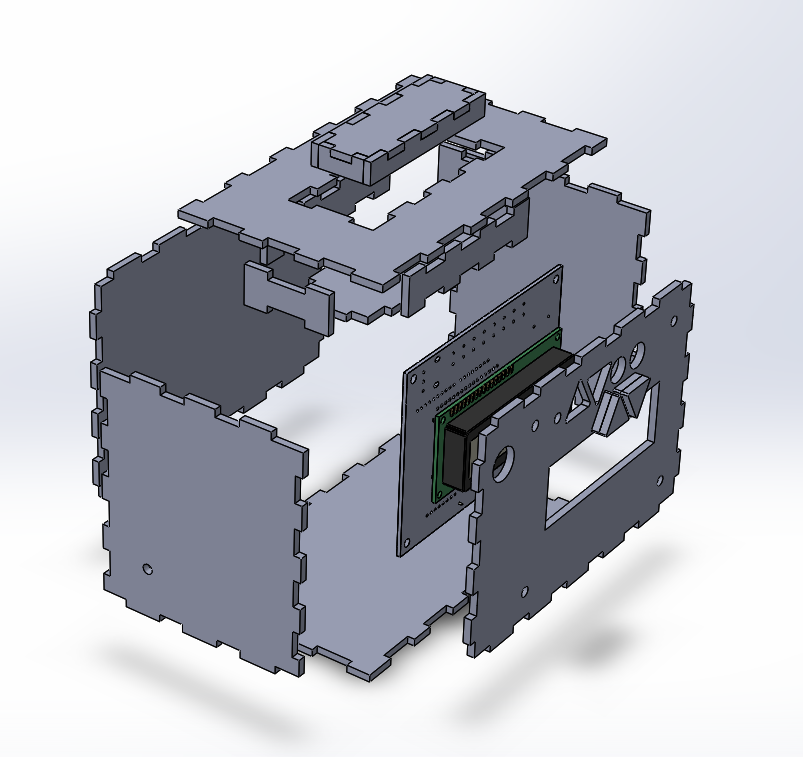
\includegraphics[width=0.8\textwidth]{AlarmExploded.png}
    \caption{Alarm Enclosure}
    \label{fig:exp}
\end{figure}
\paragraph{}
The T+/T- buttons are mounted as tall tactile switches on the PCB and are connected to the triangular buttons on the front of the enclosure. The Alarm Set and Backlight buttons are similarly connected to the circular buttons on the front of the enclosure. The cancel alarm button is a panel mount button on the left side of the front to the enclosure. The snooze button is mounted on the top of the enclosure with large cover to make pressing it easier. Dimensioned and labeled diagrams can be seen on the next two pages.

\newpage
\includepdf[landscape=true]{Clock.PDF}

\section{Hardware Test Code}
\inputminted{cpp}{..\ Code\ Test.ino}
\newpage
\section{Alarm Clock Code}
\inputminted{cpp}{..\ Code\ AlarmCode.ino}

\begin{landscape}
    \section{Project Timeline}
    \thispagestyle{empty}
    \noindent\resizebox{1.5\textwidth}{!}{
    \centering
    \begin{ganttchart}[
            vgrid,
            hgrid,
            time slot format=isodate
        ]{2020-07-06}{2020-08-19}
        \gantttitlecalendar{month=name, day}\\
        \ganttbar{Research}{2020-07-06}{2020-07-10}\\
        \ganttbar{Circuit Design}{2020-07-11}{2020-07-12}\\
        \ganttmilestone{Final Schematic Complete}{2020-07-12}\\
        \ganttbar{Software Development}{2020-07-13}{2020-07-20}\\
        \ganttbar{Software Testing}{2020-07-21}{2020-07-27}\\
        \ganttbar{PCB Design}{2020-07-13}{2020-07-24}\\
        \ganttmilestone{PCB Ordered}{2020-07-24}\\
        \ganttbar{Enclosure Design}{2020-07-25}{2020-07-27}\\
        \ganttmilestone{Project Demo}{2020-07-28}\\
        \ganttbar{Final Report}{2020-07-28}{2020-08-18}\\
        \ganttmilestone{Final Report Due}{2020-08-18}\\
        \end{ganttchart}
        }
        \vfill
{\makebox[\linewidth]{\thepage}}
\end{landscape}

\end{document}
